\chapter{Dataset}  \label{sec:dataset}

Why do we use a dataset?
- learning
- some research make them freely available to test

Describe how it was build ?

\section{Choice of the datatset}

Numerous datasets are already existing and have been made freely available. I could create my own dataset but it would have been very time consuming and I wouldn't be able to compare my results with previous scientific papers.

To choose, a couple of criteria were defined:
\begin{itemize}
    \item Preferably, it should be a recent dataset
    \item It must have a decent number of pictures (a few thousand pictures)
    \item It must be composed of a general kind of food such as worldwide, Western or Asian
    \item It must contain pictures with multi-food items
\end{itemize}

As we can see in the table \ref{table:dataset_summary}, UEC FOOD 256 is the dataset that best match our expectations.

\begin{table}
    %\setlength{\tabcolsep}{5pt} % Default value: 6pt
    \renewcommand{\arraystretch}{1.1} % Default value: 1
    \begin{tabulary}{\textwidth}{| c | C | C | C | C | C|}
        \hline
        Name & Release date & Number of pictures & Type of food & Number of classes & Multiple food items \\
        \hline
        PFID \cite{Chen2009} & 2009 & 4545 & American fast-food  & 101 & No \\
        \hline
        UEC FOOD 100 \cite{Matsuda2012a} & 2012 & 14361 & Japanese & 100  & Yes \\
        \hline
        FIDS 30 \cite{FIDS30} & 2013 & 971 & Fruit & 30 & No \\
        \hline
        ETHZ Food-101 \cite{Bossard2014} & 2014 & 101 000 & European & 100 & No \\
        \hline
        UPMC Food-101* \cite{Wang2015} & 2015 & 90 840 & European & 100 & No \\
        \hline
        UNICT-FD889 \cite{Farinella2015} & 2015 & 3 583 & World & 889 & No \\
        \hline
        FooDD \cite{ParisaPouladzadehAbdulsalamYassine2015} & 2015 & 3000 & Fruit & 23 & Yes \\
        \hline
        \textbf{UEC FOOD 256} \cite{Kawano2015} & \textbf{2015} & \textbf{31395} & \textbf{World} & \textbf{256}  & \textbf{Yes} \\ 
        \hline
    \end{tabulary}
    \caption[Summary of some available food datasets according to the criteria]{Summary of some available food datasets according to the criteria. \\
        *UPMC FOOD 101 is including the recipe for most of the pictures}
    \label{table:dataset_summary}
\end{table}

\section{UEC FOOD-100 and UEC FOOD-256}

\textbf{UEC FOOD-100} and \textbf{UEC FOOD-256} are datasets used for food localization and recognition.

The UEC FOOD-100 dataset can be found in \footnote{Dataset can be found at \url{http://foodcam.mobi/dataset100.html}}. It was created in 2012 and presented in \cite{Matsuda2012a}.

It contains 100 types of food, mainly Japanese food. Each kind is represented by at least 100 samples.

\begin{figure}[h]
    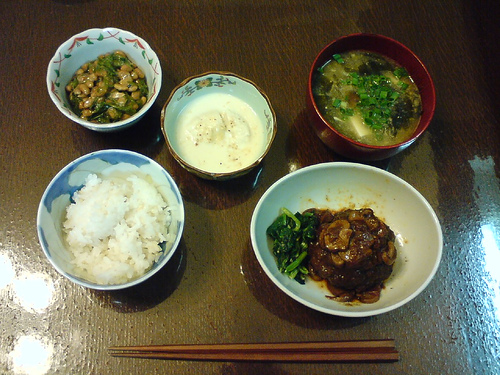
\includegraphics[width=8cm, height=8cm]{img/multiple_food_items_1}
    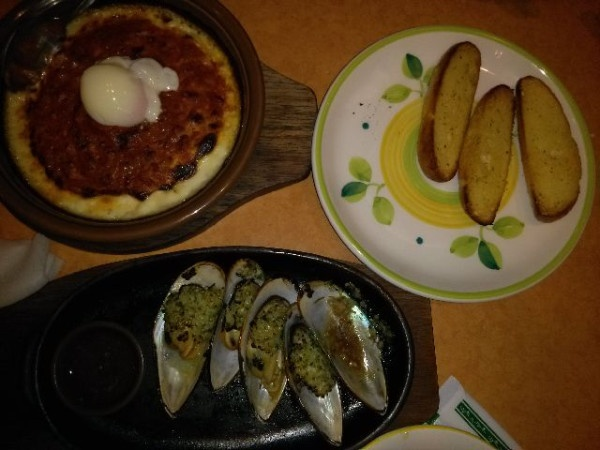
\includegraphics[width=8cm, height=8cm]{img/multiple_food_items_2}
    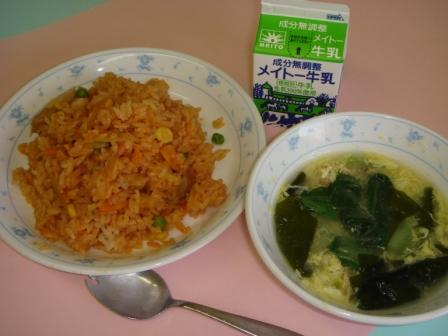
\includegraphics[width=8cm, height=8cm]{img/multiple_food_items_3}
    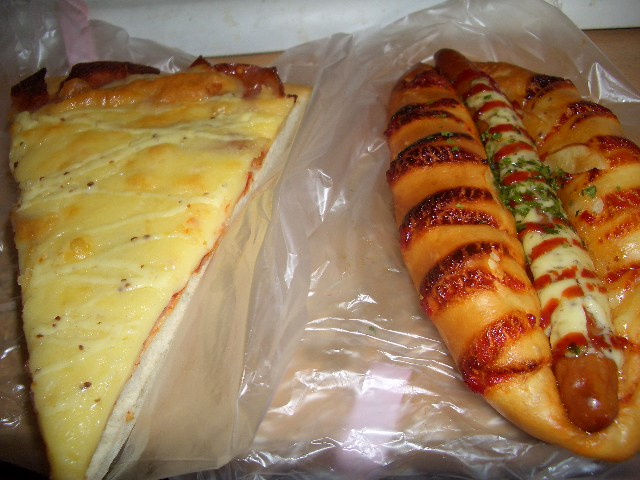
\includegraphics[width=8cm, height=8cm]{img/multiple_food_items_4}
    \caption{Pictures with multiple food items from UEC FOOD 256}
    \label{fig:presentation_multiple_food_items}
\end{figure}

As presented in figure \ref{fig:presentation_multiple_food_items}, a photo can contain more than one food items. The dataset contains files to indicate bounding boxes marking the location of a food items.

UEC FOOD-256 can be found in \footnote{Dataset can be found at \url{http://foodcam.mobi/dataset256.html}}. It was presented in \cite{Kawano2015} in 2015. It contains  the 100 types of food from UEC FOOD-100 plus 156 new ones. The pictures have been automatically  extracted from the Internet and pre-processed. 

The newly introduced food kinds are more international dishes with food from various countries such as France, Italy, the USA, China, Thailand, Vietnam, Japan and Indonesia. As for FOOD 100, every food photo has a bounding box indicating the location of the food item.

The most represented category is miso soup with 728 and rice with 620 pictures.